\subsection{Metodo del Gradiente e Metodo del Gradiente Coniugato a confronto}

Notiamo che tra i due metodi che il primo ci da come risultato delle immagini con un PSNR 
definitivamente più alto rispetto al secondo, le immagini sono qualitativamente più simili 
alle immagini originali. 

\begin{figure}[H]
    \centering
    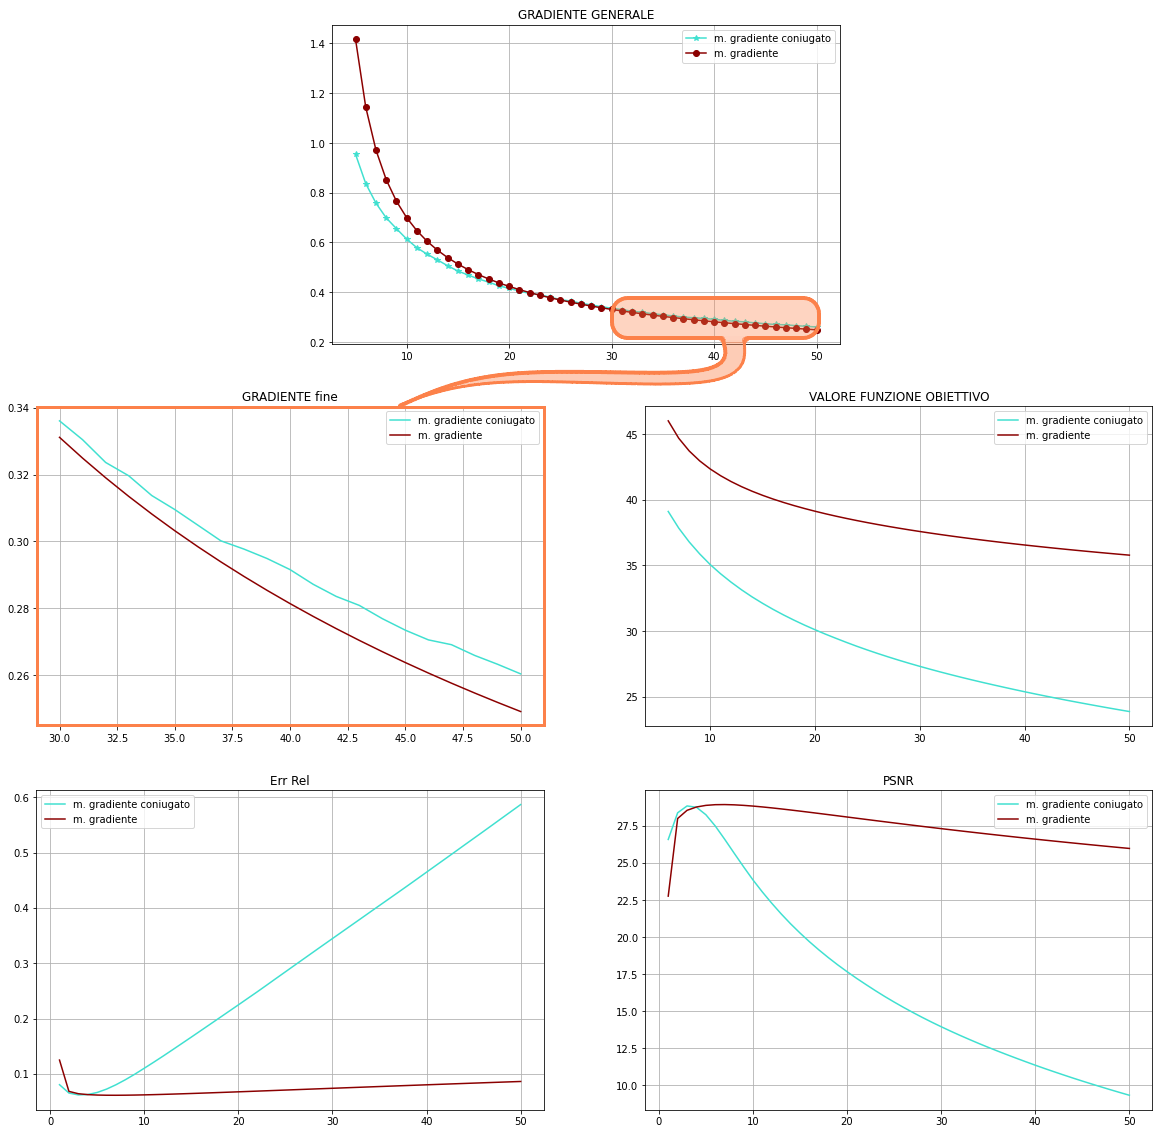
\includegraphics[width=\textwidth]{output/MGCvsMG-enph.png}
    \label{fig:MGCvsMG}
\end{figure}